\documentclass[12pt,letterpaper]{article}
\usepackage[utf8]{inputenc}

\usepackage[spanish, mexico]{babel}
\usepackage{amsmath}
\usepackage{color}
\usepackage{algorithm}
\usepackage[noend]{algpseudocode}
\renewcommand{\algorithmicrequire}{\textbf{Entrada:}}
\renewcommand{\algorithmicensure}{\textbf{Salida:}}
\usepackage{subcaption}
\usepackage{amsfonts}
\usepackage{hyperref}
 \hypersetup{
     colorlinks=true,
     linkcolor=blue,
     filecolor=blue,
     citecolor = blue,      
     urlcolor=cyan,
     }
\usepackage{amssymb}
\usepackage{listings}
\usepackage{color}

\definecolor{mygreen}{rgb}{0,0.6,0}
\definecolor{mygray}{rgb}{0.5,0.5,0.5}
\definecolor{mymauve}{rgb}{0.58,0,0.82}

\lstset{ 
  backgroundcolor=\color{white},   % choose the background color; you must add \usepackage{color} or \usepackage{xcolor}; should come as last argument
  basicstyle=\footnotesize,        % the size of the fonts that are used for the code
  breakatwhitespace=false,         % sets if automatic breaks should only happen at whitespace
  breaklines=true,                 % sets automatic line breaking
  captionpos=b,                    % sets the caption-position to bottom
  commentstyle=\color{mygreen},    % comment style
  deletekeywords={...},            % if you want to delete keywords from the given language
  escapeinside={\%*}{*)},          % if you want to add LaTeX within your code
  extendedchars=true,              % lets you use non-ASCII characters; for 8-bits encodings only, does not work with UTF-8
  firstnumber=1,                % start line enumeration with line 1000
  frame=single,	                   % adds a frame around the code
  keepspaces=true,                 % keeps spaces in text, useful for keeping indentation of code (possibly needs columns=flexible)
  keywordstyle=\color{blue},       % keyword style
  language=Octave,                 % the language of the code
  morekeywords={*,...},            % if you want to add more keywords to the set
  numbers=none,                    % where to put the line-numbers; possible values are (none, left, right)
  numbersep=5pt,                   % how far the line-numbers are from the code
  numberstyle=\tiny\color{mygray}, % the style that is used for the line-numbers
  rulecolor=\color{black},         % if not set, the frame-color may be changed on line-breaks within not-black text (e.g. comments (green here))
  showspaces=false,                % show spaces everywhere adding particular underscores; it overrides 'showstringspaces'
  showstringspaces=false,          % underline spaces within strings only
  showtabs=false,                  % show tabs within strings adding particular underscores
  stepnumber=2,                    % the step between two line-numbers. If it's 1, each line will be numbered
  stringstyle=\color{mymauve},     % string literal style
  tabsize=2,	                   % sets default tabsize to 2 spaces
  title=\lstname                   % show the filename of files included with \lstinputlisting; also try caption instead of title
}

\usepackage{amsthm}
\newtheorem{theorem}{Teorema}

\usepackage{graphicx}
\usepackage[left=2cm,right=2cm,top=2cm,bottom=2cm]{geometry}
\setlength{\parskip}{3mm}
\title{\textsc{Ajuste de curvas}}
\author{\textsc{Fabiola Vázquez}}

\setlength{\parindent}{0cm}
\renewcommand{\lstlistingname}{Código}
\floatname{algorithm}{Algoritmo}

\begin{document}
\maketitle

\hrule
\section{Introducción}
Este estudio se realiza con el software R versión 4.0.2 \cite{R}, en un cuaderno de Jupyter \cite{jupyter}. Los conjuntos de datos con los que se trabaja fueron, en mayor parte, generados con alguna función en particular. Como un ejemplo real, se consideran los datos obtenidos del INEGI \cite{inegi}, de la población de México en ciertos años.

\section{Análisis}
El objetivo es transformar ciertos conjuntos de datos a una realación lineal. Para ello se hace uso de la transformada de Tukey \cite{Laneonline}, como se muestra en la ecuación \ref{tukey_transf}. En base a esto, se implementa la función \texttt{lambda}, la cual está definida en el código \ref{lst:gc1}. Esta función toma dos conjuntos \texttt{x} y \texttt{y}, y retorna el valor de $\lambda$ que maximiza la correlación entre ellos. En dicha función, el conjunto de datos transformados es \texttt{y}.
\begin{equation} \label{tukey_transf}
\displaystyle \tilde{x}_\lambda = \begin{cases} 
 x^{\lambda}, & \text{si } \lambda >0, \\  
 \log x, & \text{si } \lambda = 0, \\  
 -x^{\lambda}, & \text{si } \lambda < 0.  
 \end{cases} 
\end{equation}

\begin{lstlisting}[label=lst:gc1,caption=Función \texttt{lambda}., frame = single]
lambda <- function (x,y){
     if (min(y) < 0){
        y<-y+abs(min(y))+0.01
    }
        
    cc <- numeric()
    lambda <- seq(-10, 10, .01)
    
    for (i in lambda){
        if (i == 0)
            cc <- c(cc, cor(x, log(y)))
        else if (i > 0)
            cc <- c(cc, cor(x, y**i))
        else
            cc <- c(cc, cor(x, -(y**i)))
    }

    return (lambda[which.max(cc)])
}
\end{lstlisting} 
Se automatiza el proceso de ajustar una curva a los conjuntos de datos con los que se trabaja, haciendo uso de la función \texttt{ajuste\_curva}, descrita en el código \ref{lst:gc2}.
\begin{lstlisting}[label=lst:gc2,caption=Función \texttt{ajuste\_curva}., frame = single]
ajuste_curva <- function(x,y){
    
    if (min(y) < 0){
        y<-y+abs(min(y))+0.01
    }
    
    lam <- lambda(x,y)
    if (abs(lam) < 0.1){
        fit <- lm(log(y)~x)
        y2 <- x*fit$coefficients[2]+fit$coefficients[1]
        plot(x,y,col=rgb(0.4,0.4,0.8,0.6),pch=16 , cex=1.3, las=1,font.lab=1, cex.lab=1.7, xlab="", ylab="")
        lines(x, exp(y2), col =rgb(0,0,0,0.9), pch=16, lwd = 2)
    }
    else  if(lam >= 0.1){
        fit <- lm (y**lam~x)
        y2 <- x*fit$coefficients[2]+fit$coefficients[1]
        plot(x,y,col=rgb(0.4,0.4,0.8,0.6),pch=16 , cex=1.3, las=1,font.lab=1, cex.lab=1.7,xlab="", ylab="")
        points(x,(y2^(1/lam)), col=rgb(0,0,0,0.5), pch=16, lwd = 2)
    }
        else{
        fit <- lm (y**lam~x)
        y2  <- -x*fit$coefficients[2]-fit$coefficients[1]
        plot(y~x,col=rgb(0.4,0.4,0.8,0.6),pch=16 , cex=1.3, las=1,font.lab=1, cex.lab=1.7,xlab="", ylab="")
        points(x, y2^(1/lam), col=rgb(0,0,0,0.5), pch=16, lwd=2)
        }
}
\end{lstlisting} 

La figura \ref{ajustecurva} contiene cuatro ejemplos de funciones a las cuales se les realiza un ajuste de curva con la función mostrada en el código \ref{lst:gc2}.

La primera función considerada es $y_1=4x^2 + r_1$, donde $r_1 \sim N(300,30000)$ es un ruido añadido para ver que tan preciso es el proceso de ajustarle una curva. Haciendo uso de la función \texttt{ajuste\_curva} se obtiene la figura \ref{cuadratica}. Considerando la función $y_2=4\sqrt{x}+10 + r_2 $, donde $r_2 \sim N(1,3)$, se obtiene la figura \ref{raiz}. Si se supone que la relación es del tipo $y_3=0.07*\exp(x) + r_3$, donde $r_3 \sim N(0, 0.2)$, se obtiene la figura \ref{exp}. 


\begin{table}
\caption{Fragmento de datos generados.}
\begin{subtable}{0.3\textwidth}
	\centering
	\caption{}
	\begin{tabular}{rrr}
  \hline
$x$ & $\qquad y=4x^2+ r_1$ & $\qquad y=4\sqrt x+10 + r_2$ \\ 
  \hline
355 & 193132.87 & 88.00 \\ 
134 & 301924.31 & 67.48 \\ 
356 & 116678.83 & 53.53 \\ 
253 & 1034167.41 & 37.23 \\ 
470 & 155104.76 & 31.39 \\ 
123 & 515293.85 & 14.45 \\ 
   \hline
\end{tabular}
	\label{a}
\end{subtable}
\hfill
\begin{subtable}{0.3\textwidth}
	\centering
	\caption{}
\begin{tabular}{rr}
  \hline
 $x$ & $\qquad y=0.07\exp (x) + r_3$ \\ 
  \hline
0.00 & -0.04 \\ 
0.05 & 0.11 \\ 
0.10 & -0.00 \\ 
0.15 & 0.15 \\ 
0.20 & -0.06 \\ 
0.25 & 0.24 \\ 
   \hline
\end{tabular}
	\label{b}
\end{subtable}
\end{table}
\subsection{Población mexicana}
Se considera la población por año en México, cuyos datos se obtuvieron del INEGI \cite{inegi}. Estos se muestran en el cuadro \ref{ine}. Usando el mismo procedimiento que en la sección precedente, se ajusta una curva a la curva de crecimiento poblacional de México. El resultado de este ajuste se observa en la figura \ref{pob}.
\begin{table}
\centering
\caption{Población total de México por año.}
\begin{tabular}{rr}
  \hline
 $\qquad \qquad$Año & $\qquad \qquad \qquad$Población \\ 
  \hline
 1910 & 15,160,369 \\ 
 1921 & 14,334,780 \\ 
 1930 & 16,552,722 \\ 
 1940 & 19,653,552 \\ 
 1950 & 25,791,017 \\ 
 1960 & 34,923,129 \\ 
 1970 & 48,225,238 \\ 
 1980 & 66,846,833 \\ 
 1990 & 81,249,645 \\ 
 1995 & 91,158,290\\ 
 2000 & 97,483,412 \\ 
 2005 & 103,263,388 \\ 
 2010 & 112,336,538 \\ 
 2015 & 119,938,473 \\ 
   \hline
\end{tabular}
\label{ine}
\end{table}

\begin{figure}
 	\centering 
 	\begin{subfigure}[b]{0.45\linewidth}
 		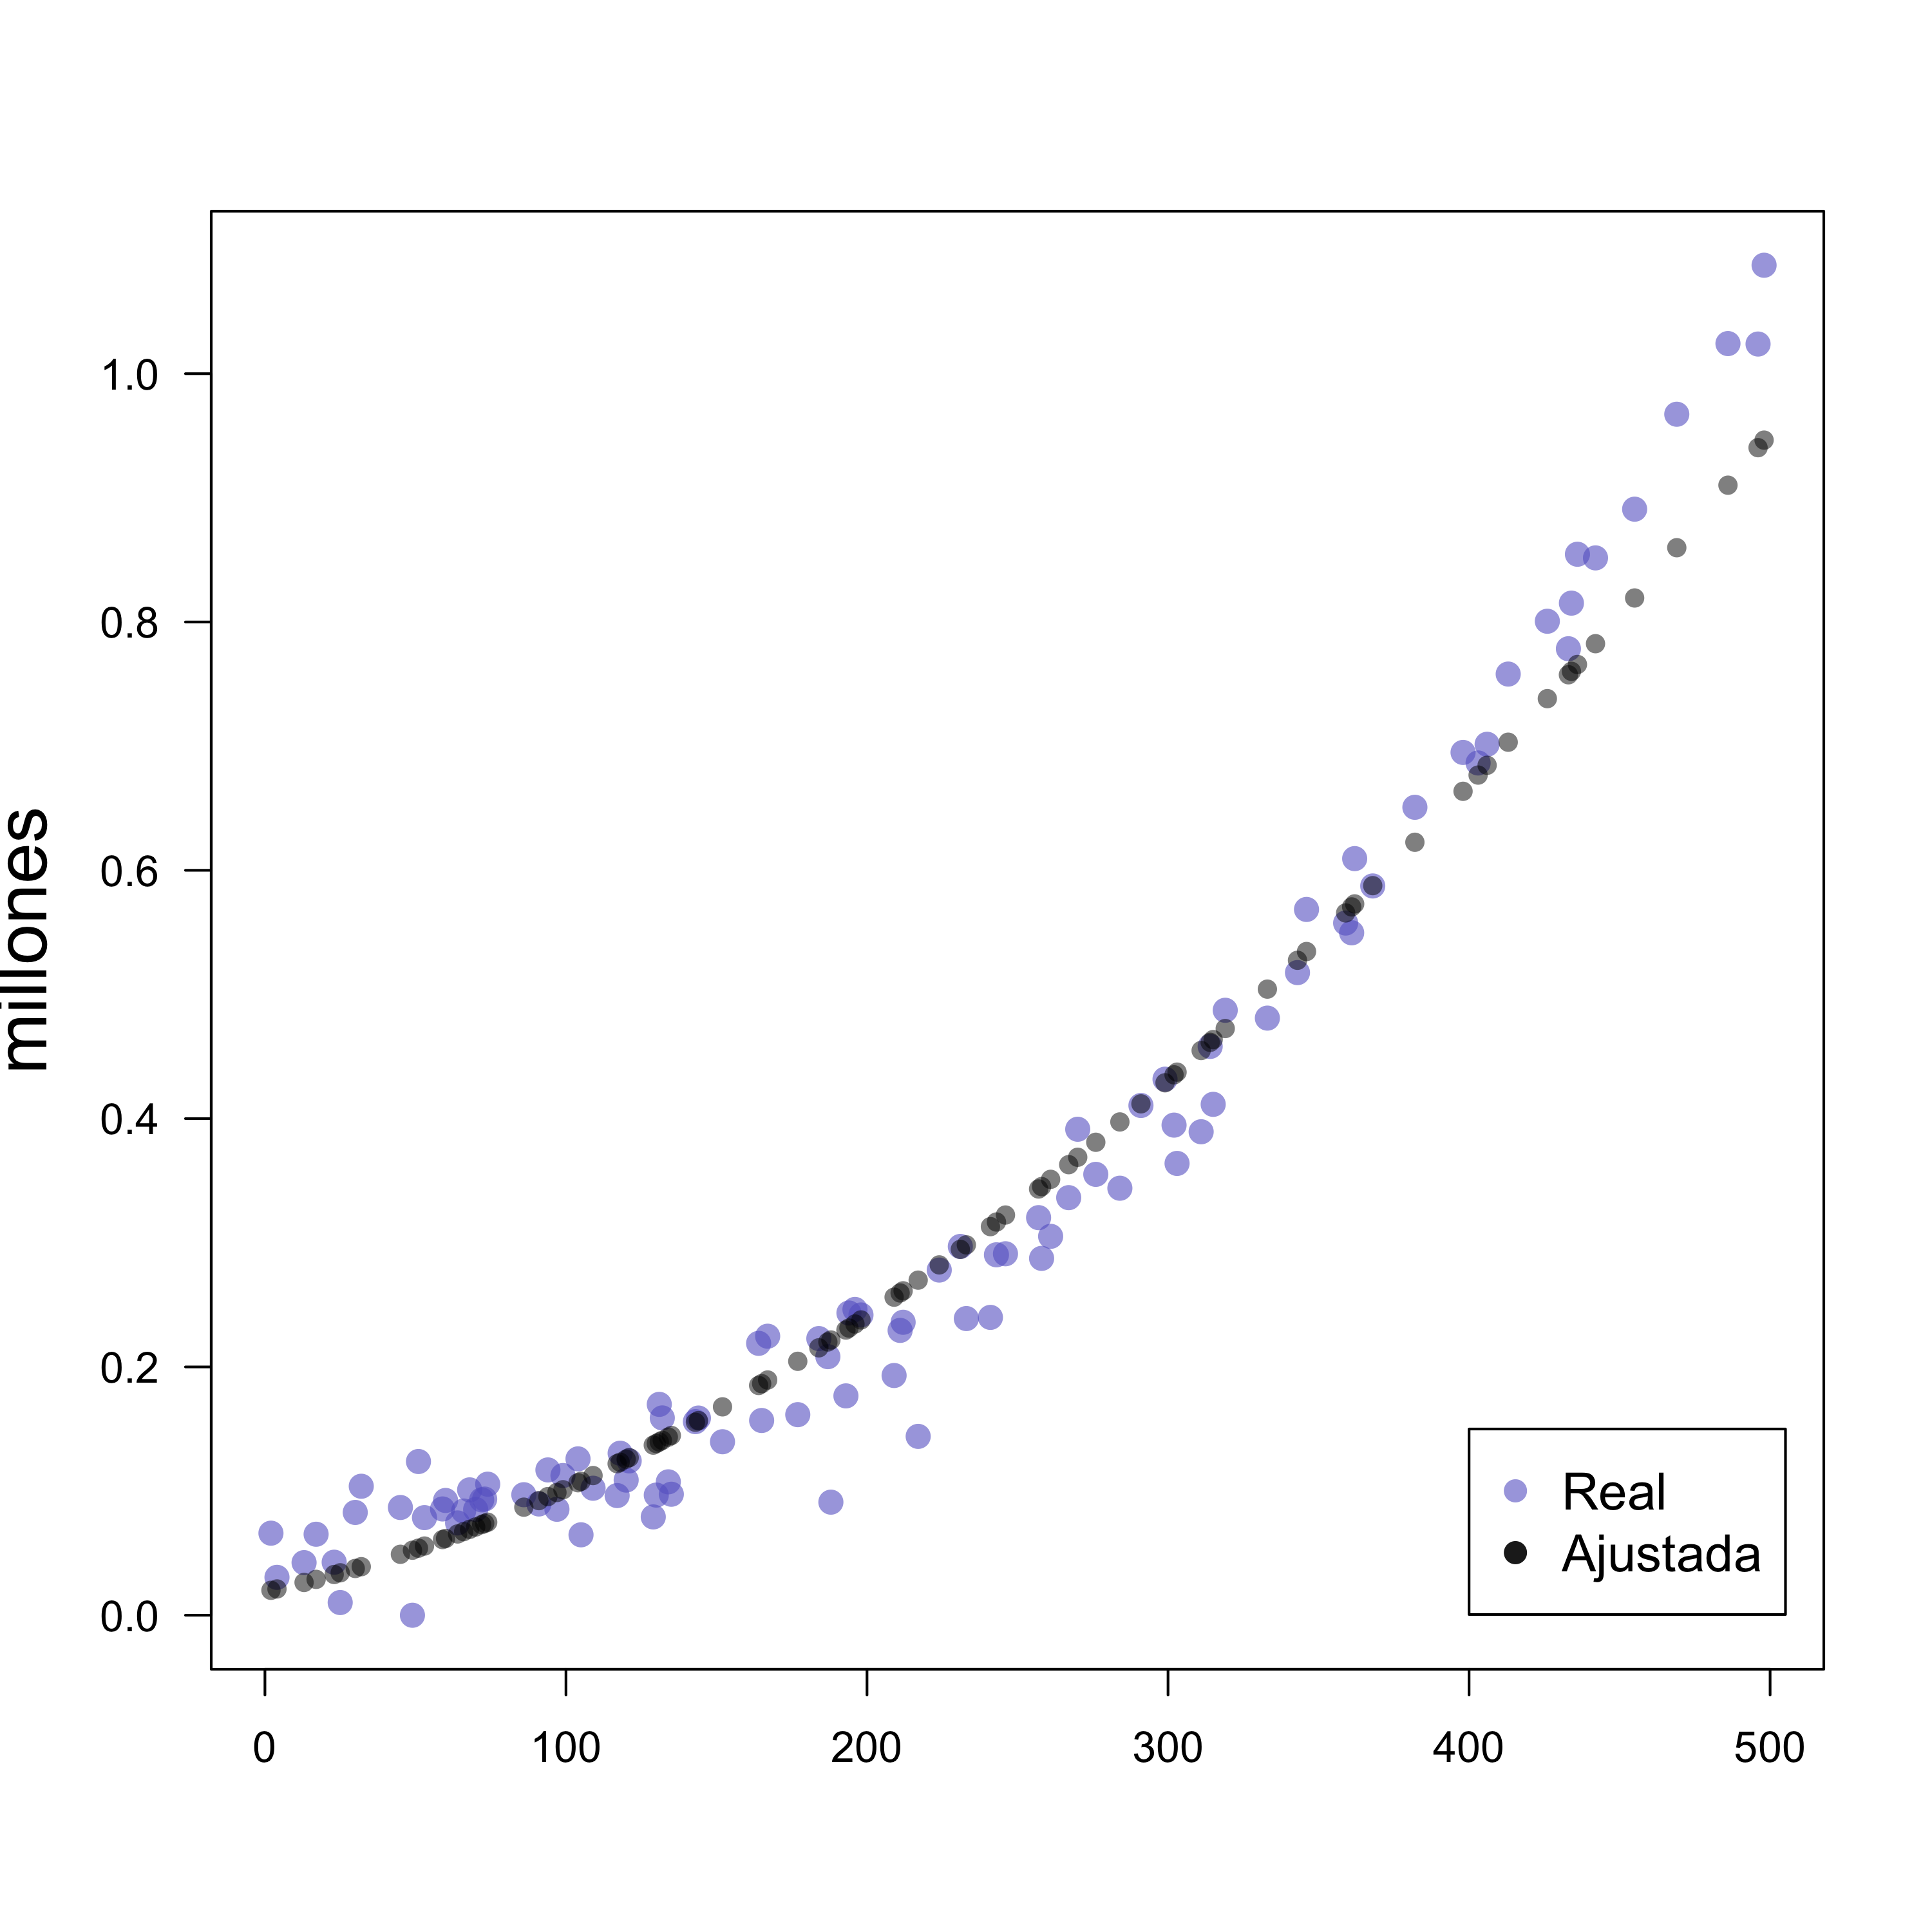
\includegraphics[width=\linewidth]{cuadratica.png} 		
 		\caption{Ajuste de una curva cuadrática.}
 		 		\label{cuadratica}
 	\end{subfigure}
 	\begin{subfigure}[b]{0.45\linewidth}
 		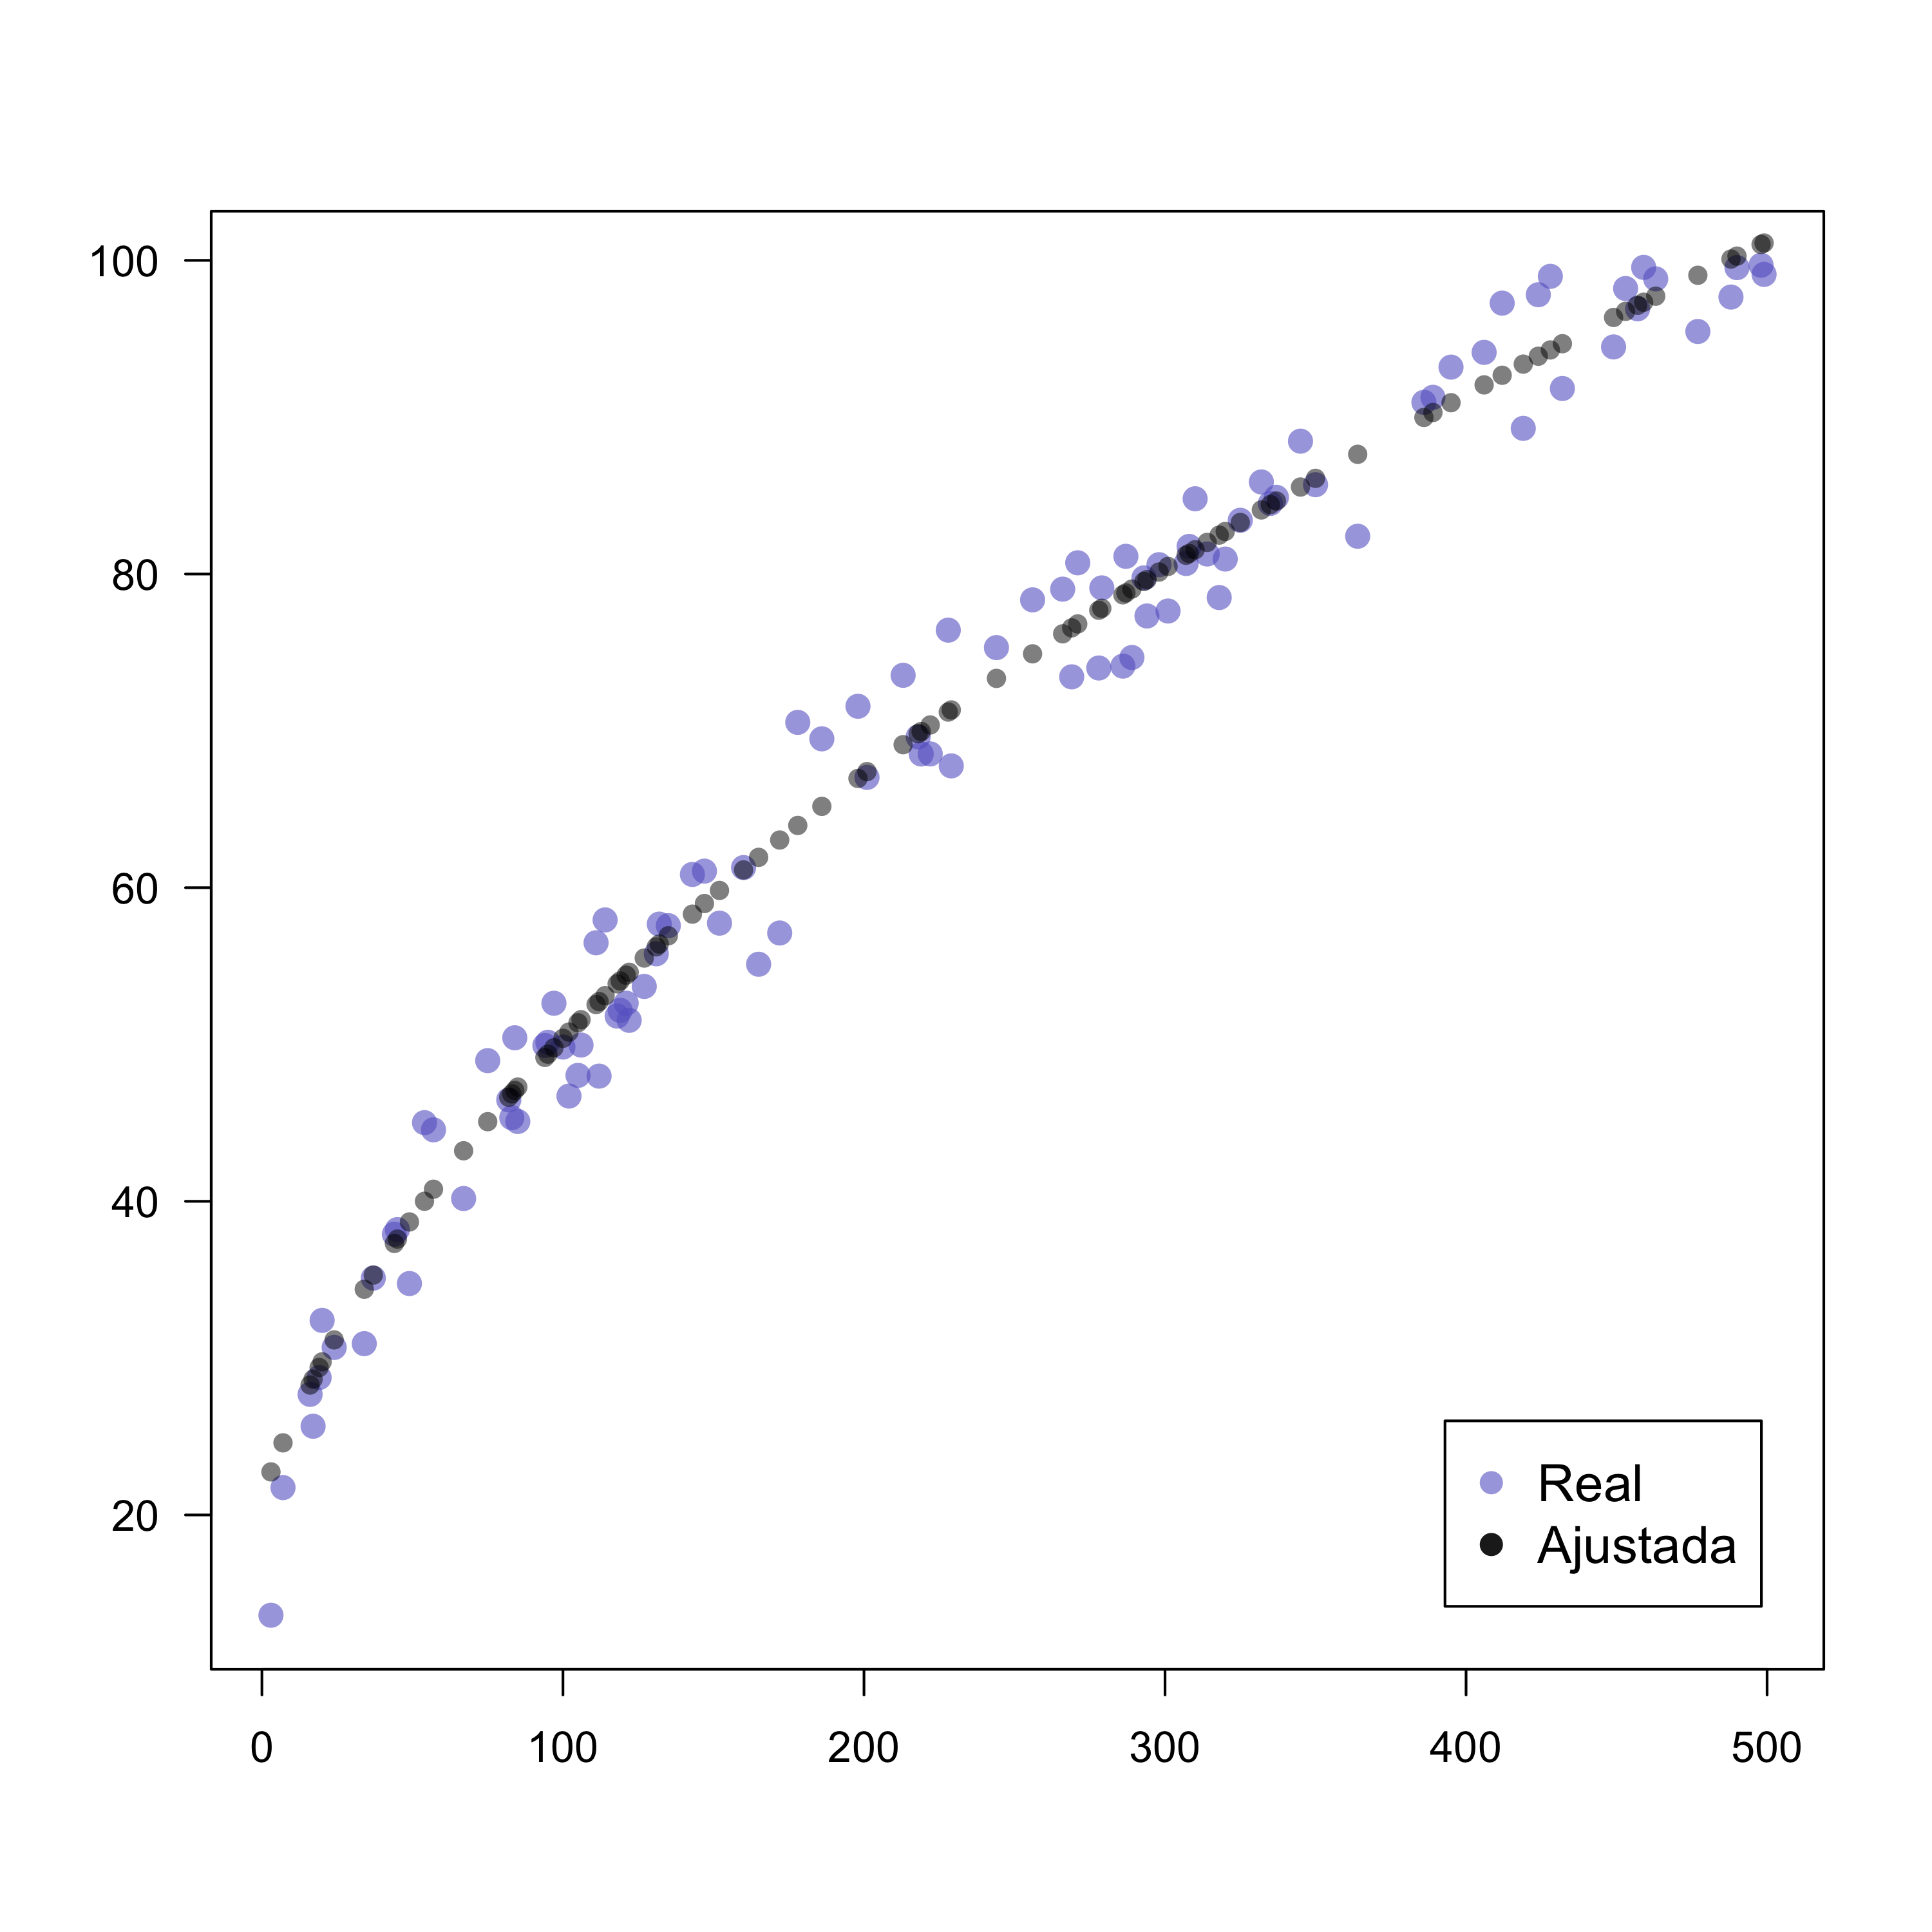
\includegraphics[width=\linewidth]{raiz.png} 		
 		\caption{Ajuste de una curva con radicales.}
 		\label{raiz}
 	\end{subfigure}
 	\begin{subfigure}[b]{0.45\linewidth}
 		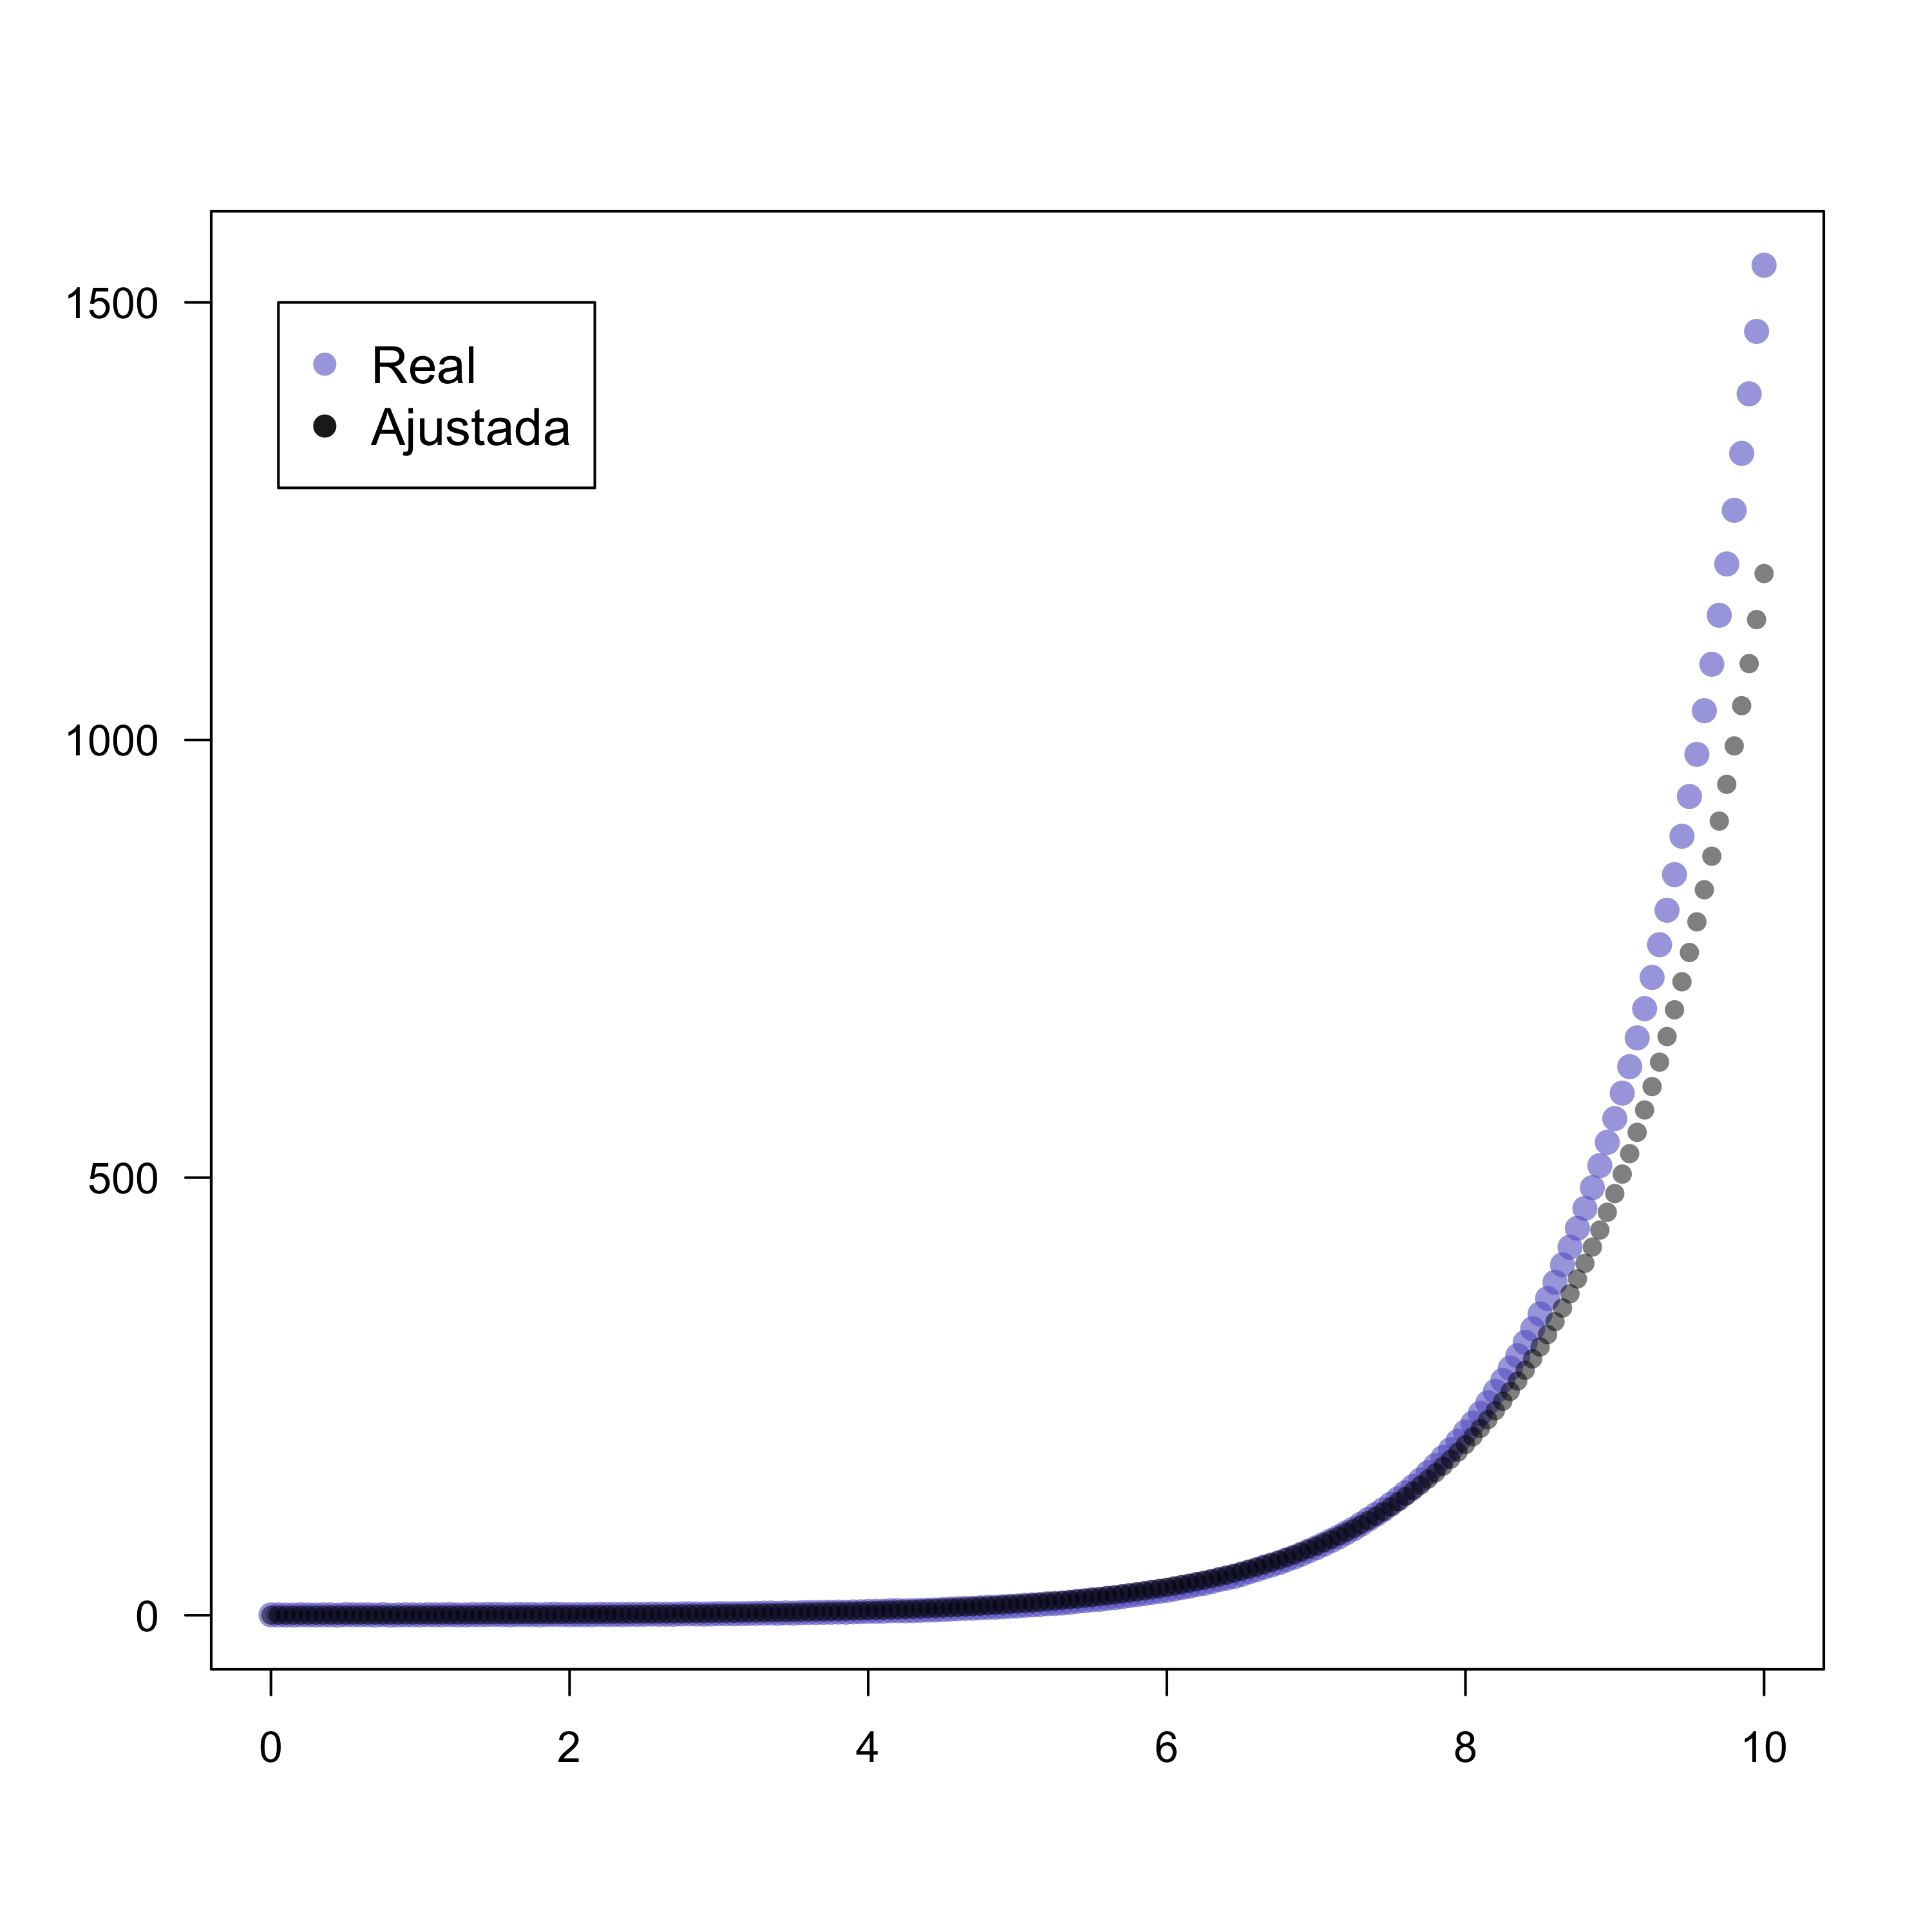
\includegraphics[width=\linewidth]{exponencial.png} 		
 		\caption{Ajuste de una curva exponencial.}
 		\label{exp}
 	\end{subfigure}
 	\begin{subfigure}[b]{0.45\linewidth}
 		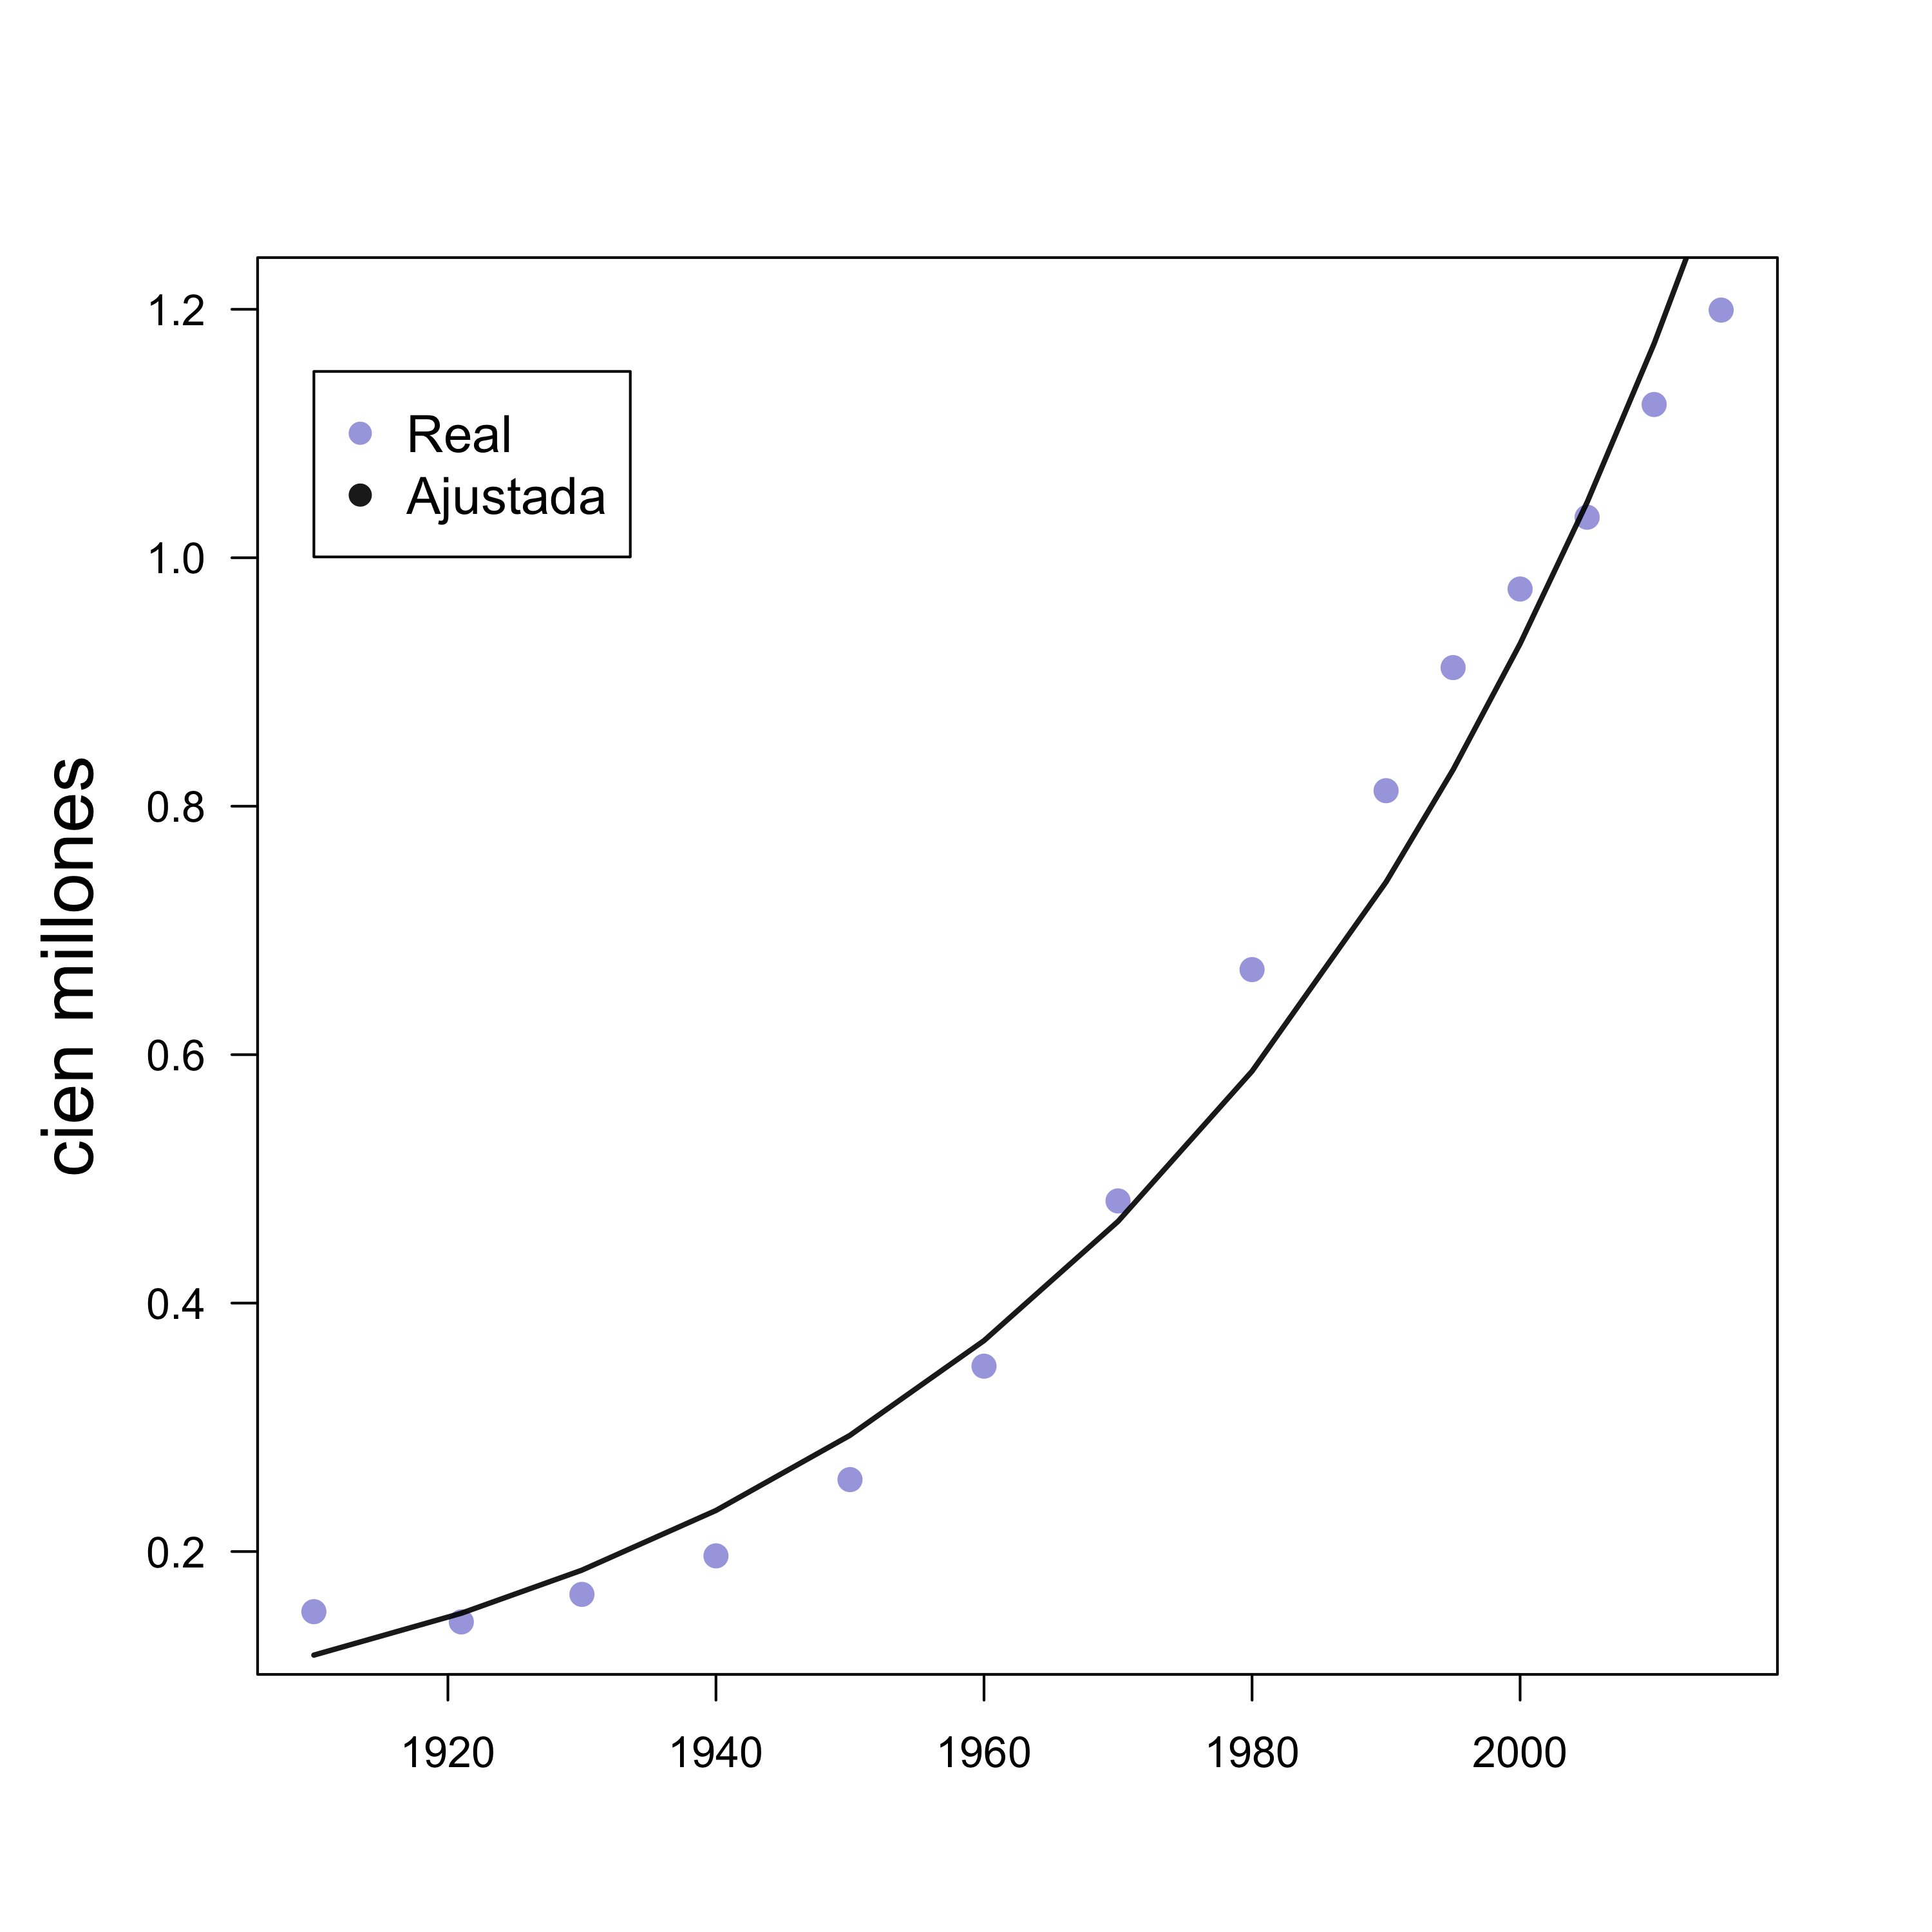
\includegraphics[width=\linewidth]{poblacion.png} 		
 		\caption{Ajuste de datos obtenidos del INEGI.}
 		\label{pob} 		
 	\end{subfigure}
 	 	\caption{Ajuste de curvas con la función \texttt{ajuste\_curva}.} 
 	 		\label{ajustecurva}
\end{figure}

\subsection{Aproximación de polinomios}
Se consideran los polinomios $y_1=0.1x^3 - 0.5x^2 - x + 10 + r_3$ y $y_2=0.1x^5 +0.5x^3 - 0.4x^2 - 0.3x + 20 + r_4$. Un fragmento de los datos generados con estas funciones se muestra en el cuadro \ref{polis}. Para ajustar curvas a este tipo de funciones \cite{scatterplot} se trabaja con la función \texttt{lm(y $\sim$ w)}, donde \texttt{w} es la suma de las diferentes potencias de \texttt{x} con las que cuenta el polinomio a ajustar. Por ejemplo, en el primer caso, la función utilizada es \texttt{lm(y $\sim$ x + I(x$\wedge$2) + I(x$\wedge$3))} ya que es un polinomio de grado tres. La figura \ref{polinomio1} muestra, en línea roja, la curva ajustada al polinomio $y_1$ y la figura \ref{polinomio2}, la curva ajustada al polinomio $y_2$.
\begin{table}
\caption{Fragmento de datos generados por polinomios.}
\begin{subtable}{0.3\textwidth}
	\centering
	\caption{}
	\begin{tabular}{rr}
  \hline
$x$ & $ y=0.1x^3 - 0.5x^2 - x + 10 + r_3$  \\ 
  \hline
-8.05 & -64.49 \\ 
-5.07 & -12.48 \\ 
-5.24 & -8.56 \\ 
-8.28 & -74.01 \\ 
4.26 & 5.58 \\ 
-8.25 & -55.56 \\ 
   \hline
\end{tabular}
	\label{c}
\end{subtable}$\qquad \qquad \qquad \quad$\begin{subtable}{0.3\textwidth}
	\centering
	\caption{}
\begin{tabular}{rr}
  \hline
 $x$ & $ y=0.1x^5 +0.5x^3 - 0.4x^2 - 0.3x + 20 + r_4$ \\ 
  \hline
-413.88 & 3,820,341,696,610.39 \\ 
-673.99 & -15,187,467,243,469.90 \\ 
817.58 & 42,608,724,664,634.36 \\ 
949.80 & 70,229,446,578,344.88 \\ 
445.92 & 1,198,984,909,305.33 \\ 
118.82 & 5,554,388,743,064.81 \\
   \hline
\end{tabular}
	\label{b}
\end{subtable}
\label{polis}
\end{table}

\begin{figure}
 	\centering 
 	\begin{subfigure}[b]{0.45\linewidth}
 		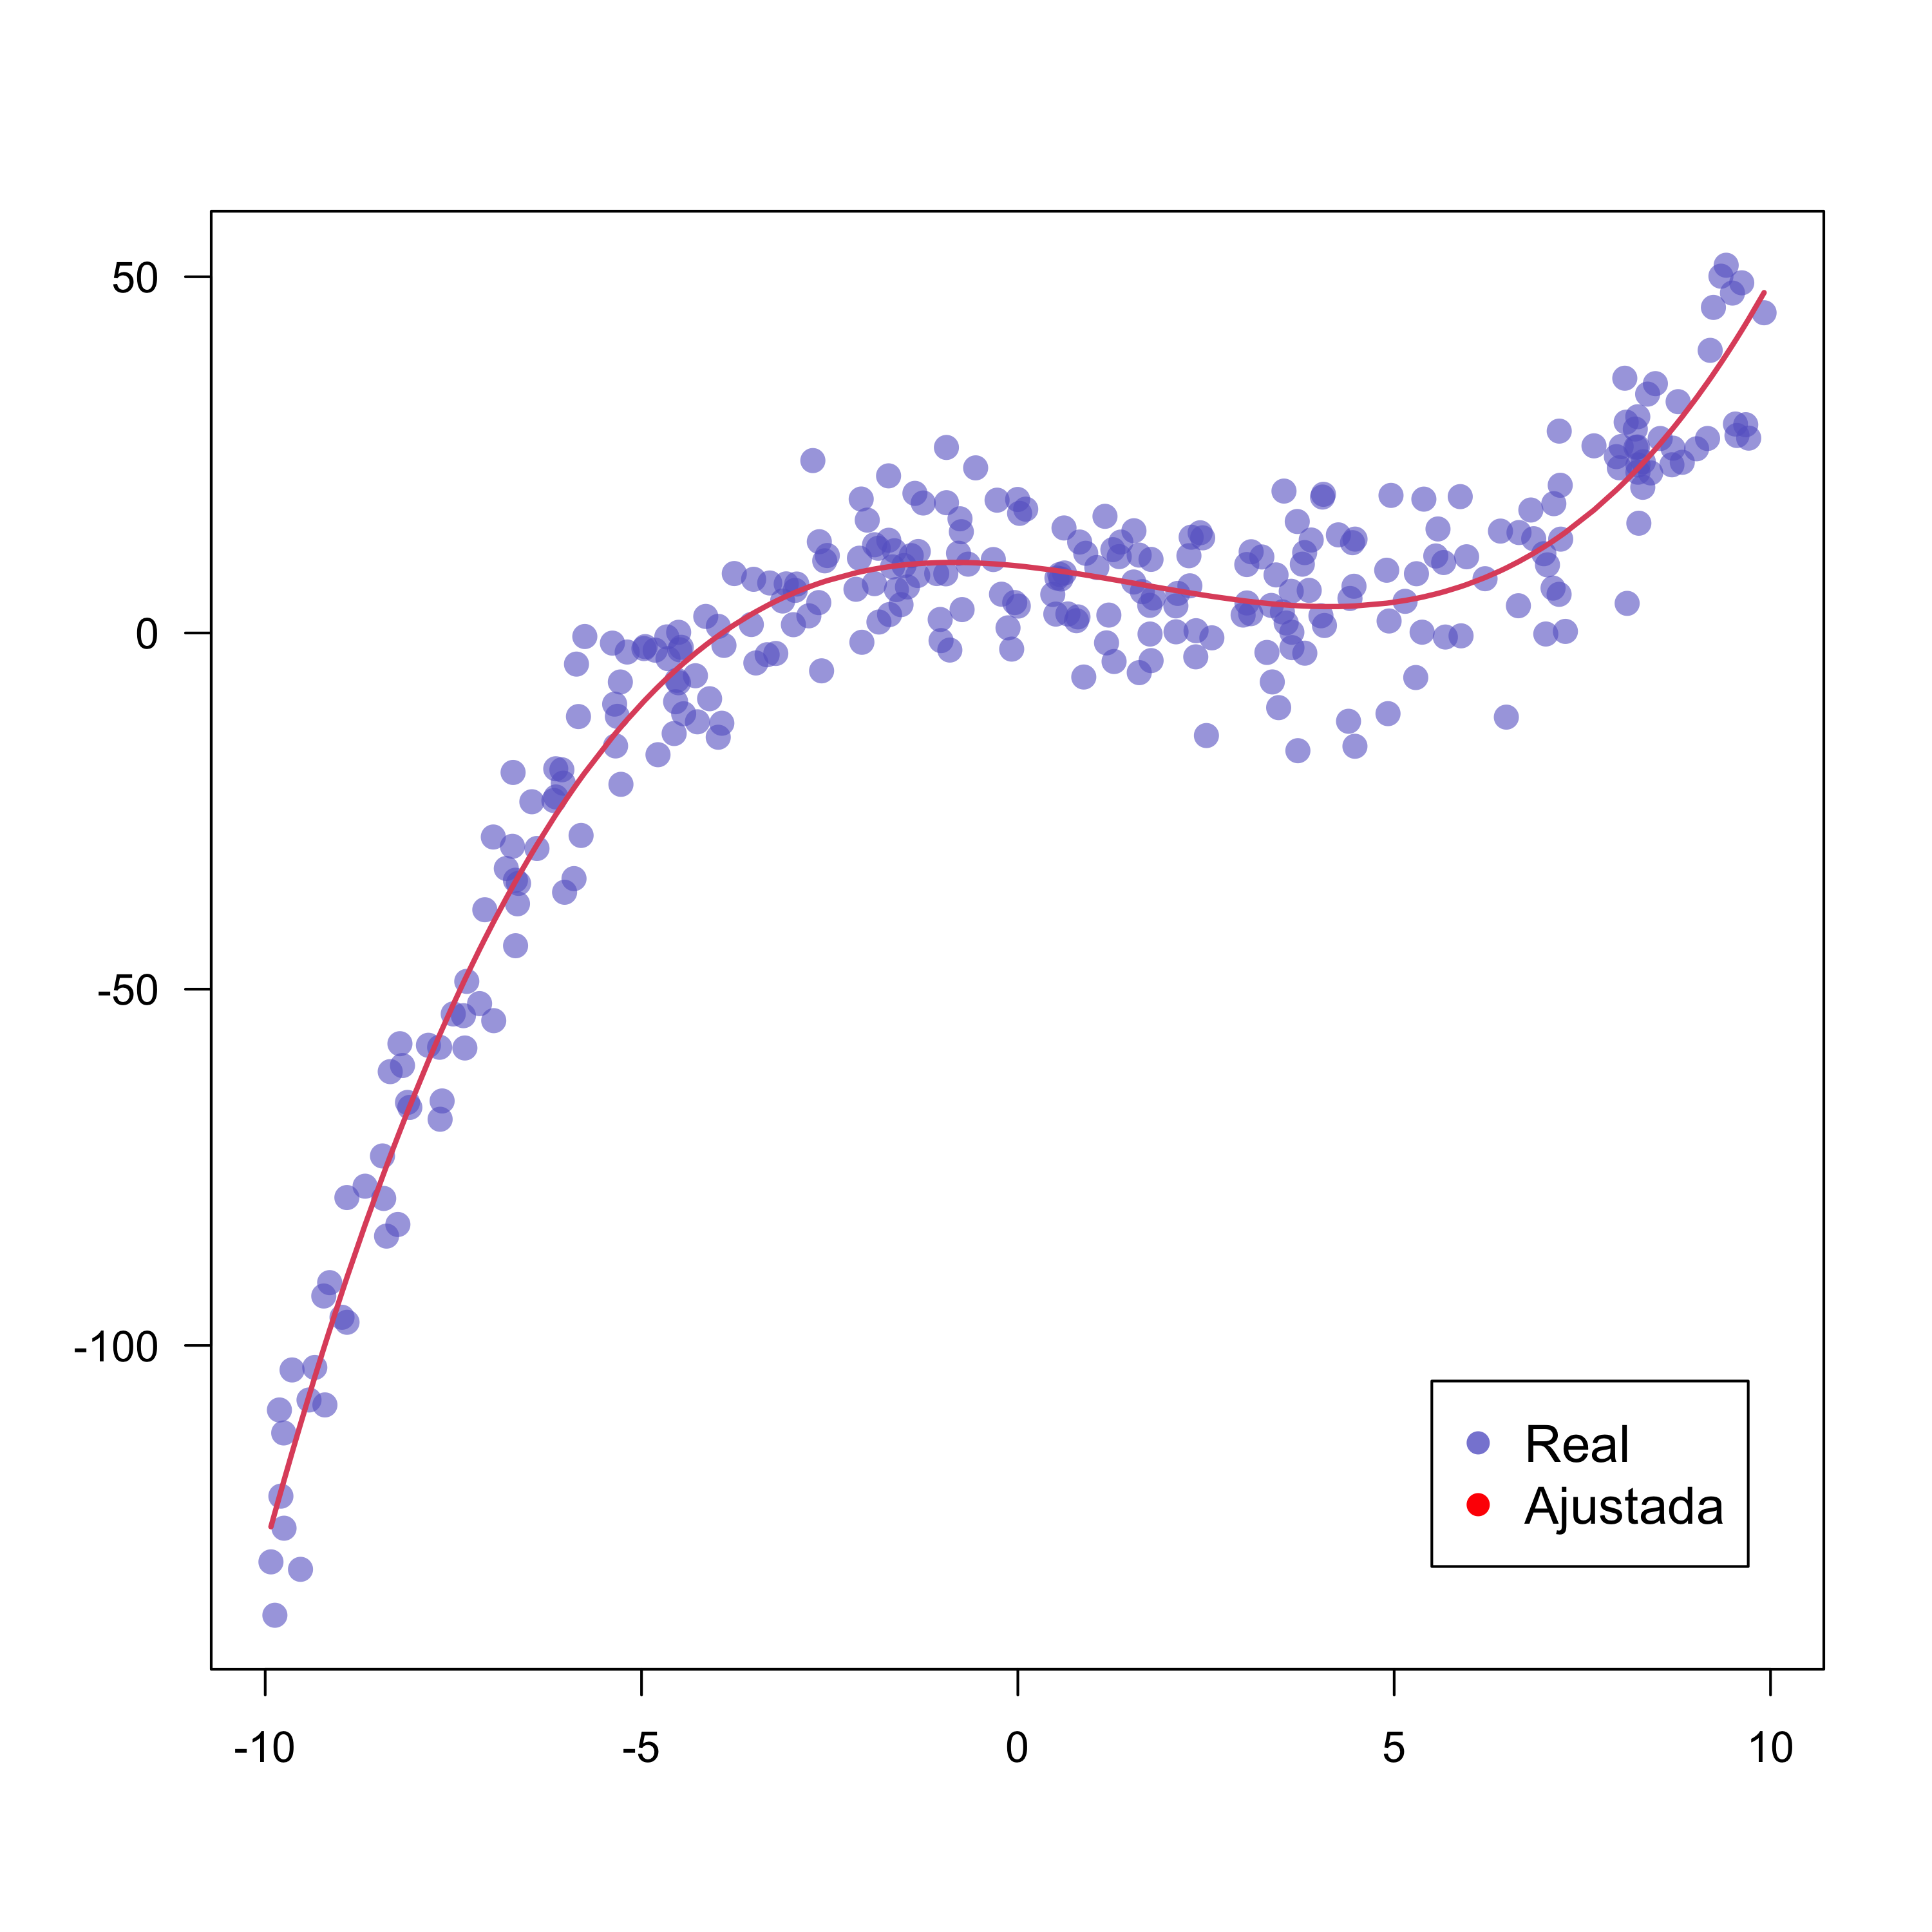
\includegraphics[width=\linewidth]{polinomio1.png} 		
 		\caption{Ajuste de una curva polinomial de grado dos.}
 		 		\label{polinomio1}
 	\end{subfigure} \quad 
 	\begin{subfigure}[b]{0.45\linewidth}
 		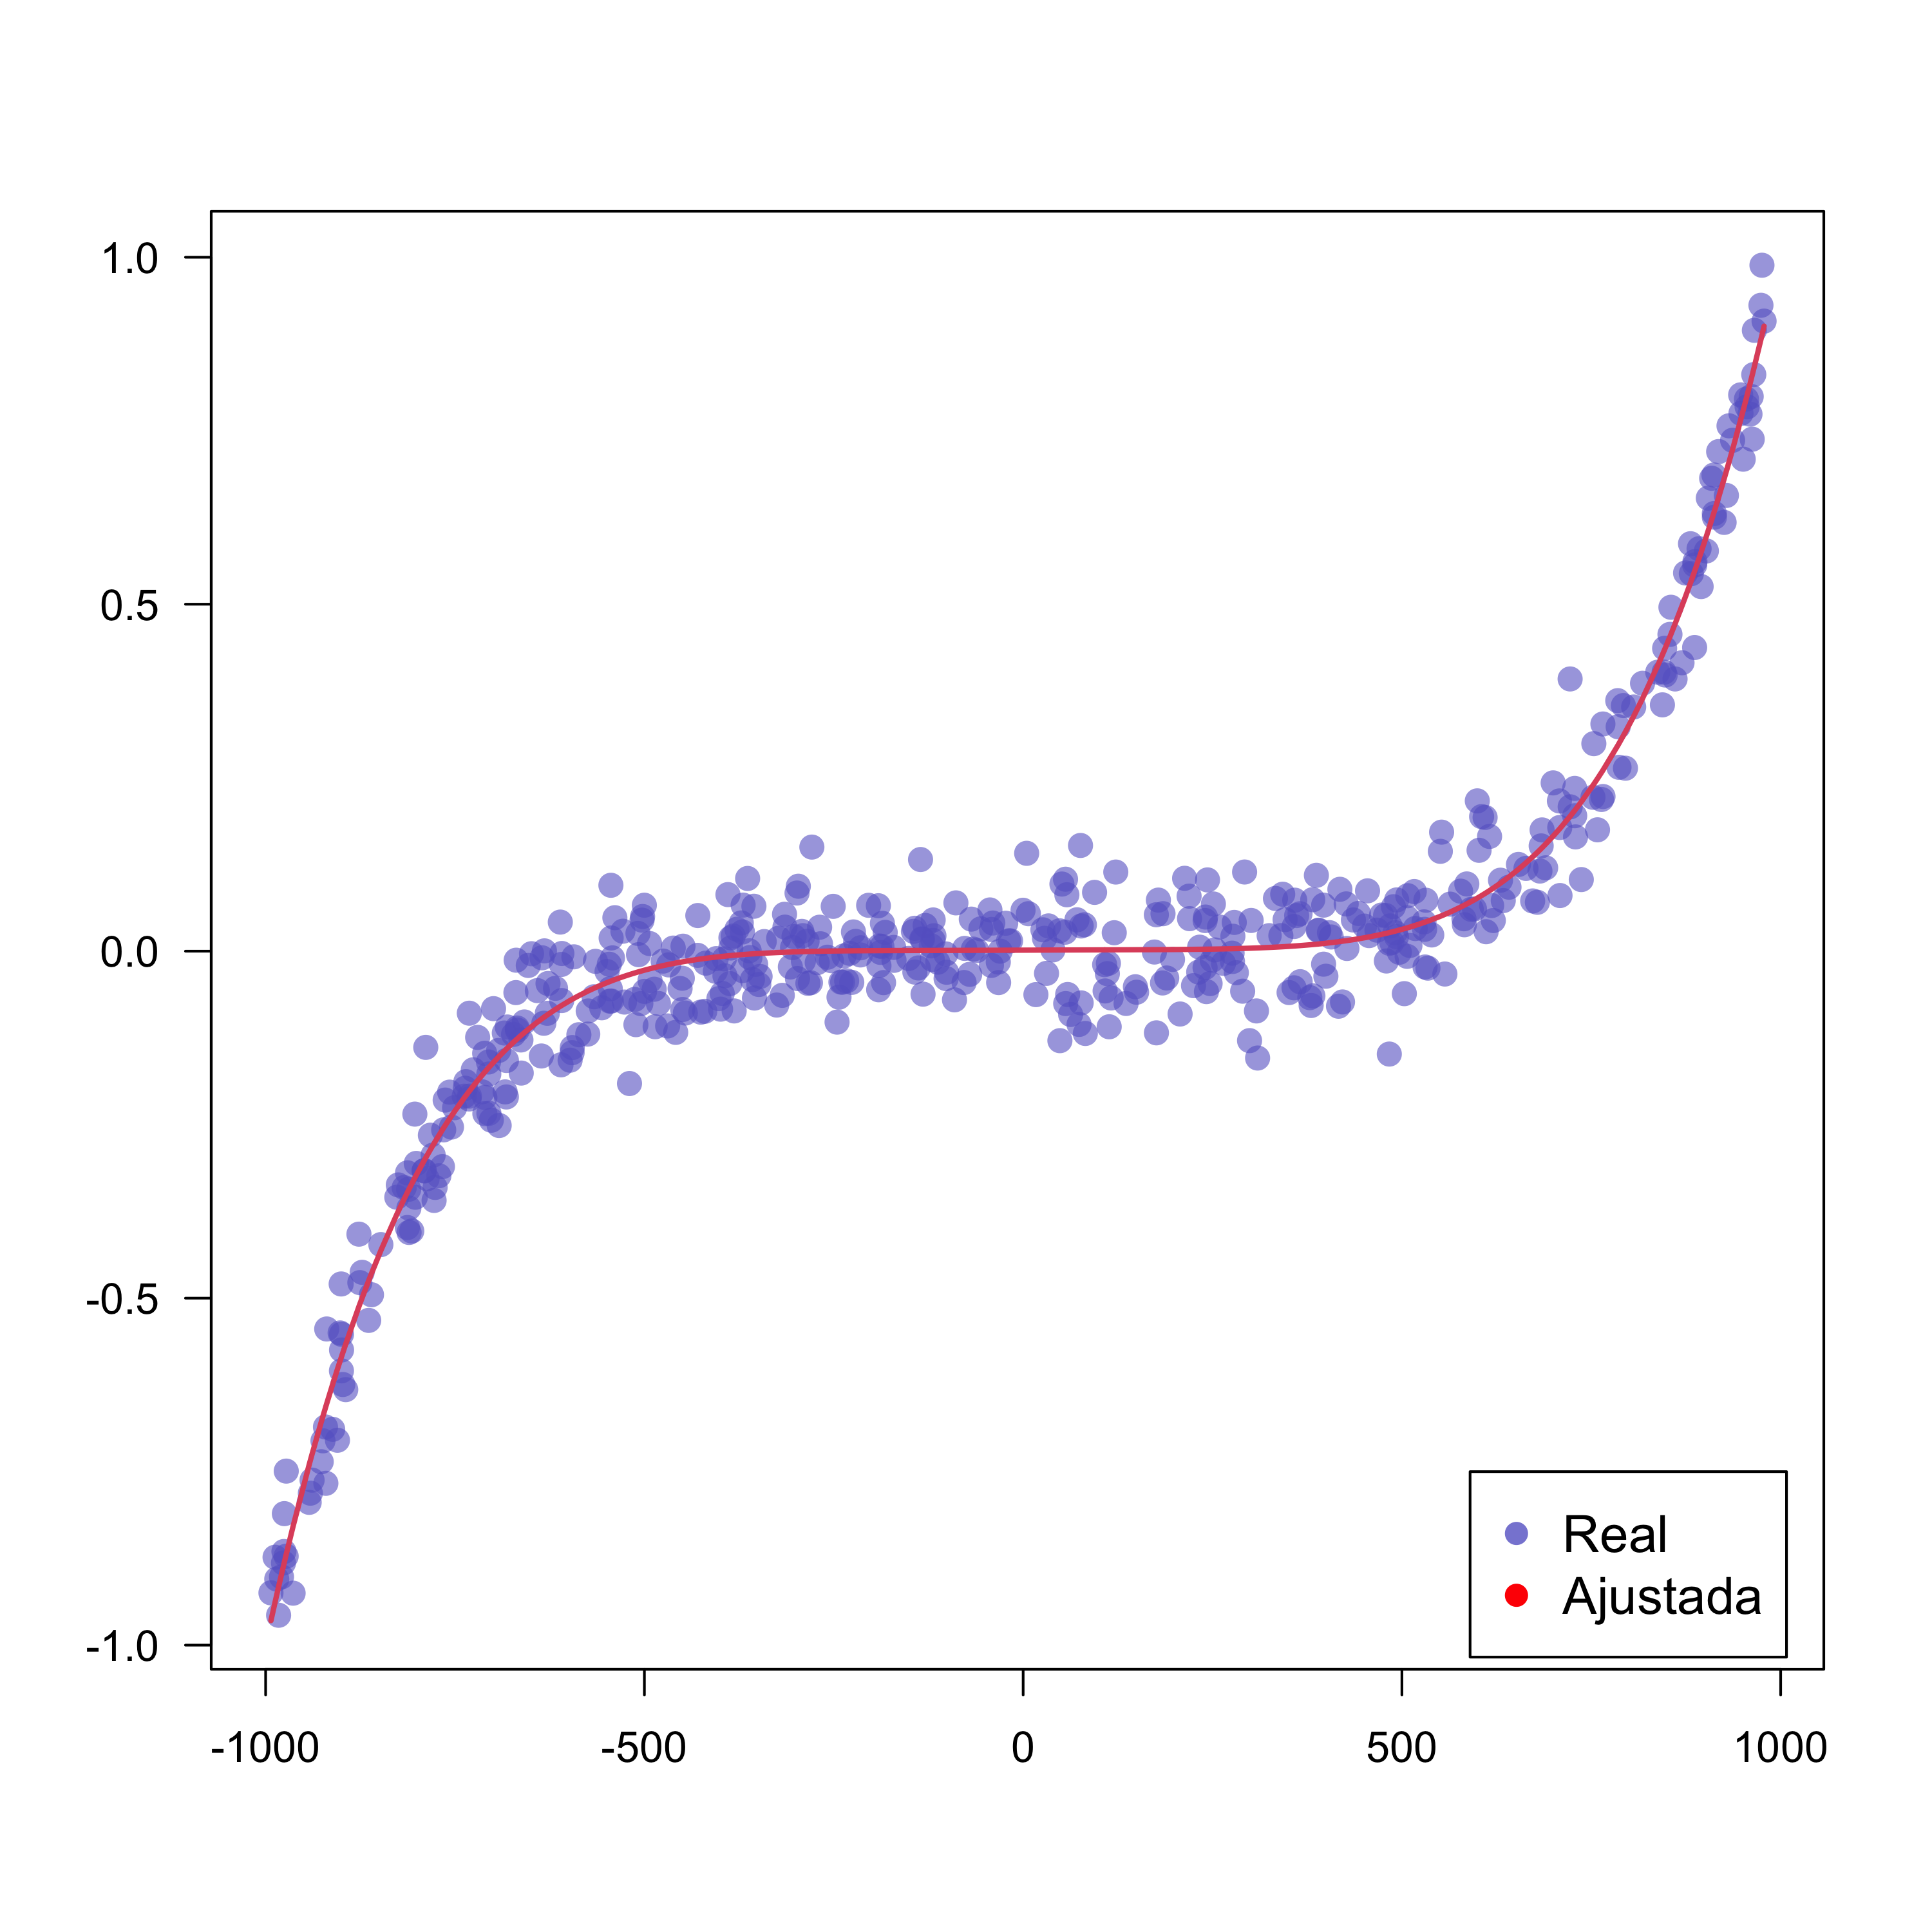
\includegraphics[width=\linewidth]{polinomio2.png} 		
 		\caption{Ajuste de una curva polinomial de grado cinco.}
 		\label{polinomio2}
 	\end{subfigure}

 	 	\caption{Ajuste de curvas con la función \texttt{ajuste\_curva}.} 
 	 		\label{polinomios}
\end{figure}

\subsection{Multivariada}
Se considera una función de tres variables independientes $y = x_1 + .4\log(x_2) + 4x_3$. Haciendo uso de la función \texttt{lm}, se obtienen los siguientes resultados. 
\begin{verbatim}
Call:
lm(formula = y ~ x1 + log(x2) + x3)

Coefficients:
(Intercept)         x1        log(x2)           x3  
  8.402e-13    1.000e+00    4.000e-01    4.000e+00 
\end{verbatim}

\bibliographystyle{plain} 
\bibliography{Referencias}


\end{document} 